% Supplementary_figures.tex
%\documentclass[preprint,12pt]{elsarticle}
\documentclass[jpm,supfile,submit,moreauthors,pdftex]{Definitions/mdpi}

% major revision and answer question (3 reviewers)
%Sunday, January 24⋅22:30 – 22:55
%Daily, until Jan 29, 2021

\renewcommand{\figurename}{Supplementary Figure } %S

% \usepackage{multirow}
\usepackage{graphicx}
\usepackage[table,xcdraw]{xcolor}

\usepackage{siunitx} % for  1e-10 scientific notation
\usepackage{array}
\usepackage{ragged2e}
\usepackage{rotating}
\usepackage{tabularx}
\usepackage{makecell}
% \usepackage{array}
\usepackage{multirow}
\usepackage{colortbl}
\usepackage{hhline}

% mark in blue or red
\usepackage{xcolor}

\newenvironment{MyColorPar}[1]{%
    \leavevmode\color{#1}\ignorespaces%
}{%
}%

\usepackage{outlines}

%%% for abbreviations, or acronyms
\usepackage[acronym, nopostdot]{glossaries} 
%\usepackage{glossary-inline}
%\newenvironment{abbreviation}
%\makeglossaries %https://tex.stackexchange.com/questions/110095/list-of-acronyms-is-not-displayed
\newacronym{fdr}{FDR}{false discovery rate}
\newacronym{hpa}{HPA}{the Human Protein Atlas}
\newacronym{hnscc}{HNSCC}{head and neck squamous cell carcinoma}
\newacronym{tcga}{TCGA}{the Cancer Genome Atlas}
\newacronym{tcpa}{TCPA}{the Cancer Proteome Atlas}
\newacronym{rna}{RNA}{ribonucleic acid}
\newacronym{rnaseq}{RNA-Seq}{RNA sequencing}
\newacronym{lncrna}{lncRNA}{long non-coding RNA}
%\newacronym{km}{KM}{Kaplan-Meier}
\newacronym{rppa}{RPPAs}{reverse-phase protein arrays}
\newacronym{rpma}{RPMA}{reverse-phase protein lysate microarray}

\newacronym{mmp}{MMP}{matrix metalloproteinase}
 %DKK1, CAMK2N1, STC2, PGK1, SURF4, USP10, NDFIP1, FOXA2, STIP1, and DKC1
 %ZNF557, ZNF266, IL19, MYO1H, FCGBP, LOC148709, EVPLL, PNMA5, KIAA1683, and NPB

\newacronym{DKK1}{DKK1}{dickkopf WNT signaling pathway inhibitor 1} 
\newacronym{CAMK2N1}{CAMK2N1}{calcium/calmodulin dependent protein kinase II inhibitor 1} 
\newacronym{STC2}{STC2}{stanniocalcin 2} 
\newacronym{PGK1}{PGK1}{phosphoglycerate kinase 1} 
\newacronym{SURF4}{SURF4}{surfeit 4} 
\newacronym{USP10}{USP10}{ubiquitin specific peptidase 10} 
\newacronym{NEDD4}{NEDD4}{neural precursor cell expressed, developmentally down-regulated 4}
\newacronym{NDFIP1}{NDFIP1}{NEDD4 family interacting protein 1} 
\newacronym{FOXA2}{FOXA2}{forkhead box A2} 
\newacronym{STIP1}{STIP1}{stress-induced-phosphoprotein 1} 
\newacronym{DKC1}{DKC1}{dyskeratosis congenita 1, dyskerin} 

\newacronym{ZNF557}{ZNF557}{zinc finger protein 557} 
\newacronym{ZNF266}{ZNF266}{zinc finger protein 266} 
\newacronym{IL19}{IL19}{interleukin 19} 
\newacronym{MYO1H}{MYO1H}{myosin 1H} 
\newacronym{FCGBP}{FCGBP}{Fc fragment of IgG binding protein} 
\newacronym{LOC148709}{LOC148709}{LncRNA LOC148709} 
\newacronym{EVPLL}{EVPLL}{envoplakin-like protein} 
\newacronym{PNMA5}{PNMA5}{paraneoplastic antigen like 5} 
%\newacronym{KIAA1683}{KIAA1683}{IQCN, IQ Motif Containing N} 
\newacronym{IQCN}{IQCN}{IQ motif containing N} % previous name KIAA1683
% "IQ" refers to the first two amino acids of the motif: isoleucine (commonly) and glutamine (invariably)
\newacronym{NPB}{NPB}{neuropeptide B} 

 \newacronym{rt}{RT}{radiation therapy}
 \newacronym{nccn}{NCCN}{National Comprehensive Cancer Network}
 \newacronym{hif}{HIF}{hypoxia-inducible factor}
 \newacronym{egfr}{EGFR}{epidermal growth factor receptor}
 \newacronym{ras}{RAS}{rat sarcoma}
 \newacronym{hras}{HRAS}{Harvey rat sarcoma viral oncoprotein}
 \newacronym{erk}{ERK}{extracellular signal-regulated kinases}
 \newacronym{us}{US}{United States}
 \newacronym{fda}{FDA}{Food and Drug Administration}
 \newacronym{tpf}{Tax-PF}{docetaxel, cisplatin, and 5-fluorouracil}
 \newacronym{tki}{TKI}{tyrosine kinase inhibitor}
 \newacronym{her}{HER}{human epidermal growth factor receptor}
 \newacronym{ici}{ICI}{immune-checkpoint inhibitor}
 \newacronym{ctla4}{CTLA-4}{cytotoxic T lymphocyte antigen 4}
 \newacronym{pd1}{PD-1}{programmed death 1}
 \newacronym{pdl1}{PD-L1}{programmed death ligand 1}
 \newacronym{tim3}{TIM-3}{T-cell immunoglobulin mucin protein 3}
 \newacronym{lag3}{LAG-3}{lymphocyte activation gene 3}
 \newacronym{ifng}{IFN-$\gamma$}{interferon gamma}
 \newacronym{tigit}{TIGIT}{T cell immunoglobin and immunoreceptor tyrosine-based inhibitory motif}
 \newacronym{gitr}{GITR}{glucocorticoid-induced tumor necrosis factor receptor}
 \newacronym{vista}{VISTA}{V-domain Ig suppressor of T-cell activation}
 \newacronym{tmsb4x}{TMSB4X}{thymosin beta-4 X-linked}
 \newacronym{emt}{EMT}{epithelial-mesenchymal-transition}
 \newacronym{gdc}{GDC}{Genomic Data Commons}
 \newacronym{nci}{NCI}{the National Cancer Institute}
 \newacronym{gdac}{GDAC}{Genome Data Analysis Center}
 \newacronym{rest}{REST}{Representational State Transfer} 
 \newacronym{api}{API}{Application Programmable Interface}
\newacronym{grch38}{GRCh38}{Genome Reference Consortium Homo sapiens genome assembly 38}
\newacronym{fpkm}{FPKM}{Fragments per kilobase per million reads mapped}
\newacronym{rsem}{RSEM}{RNA-Seq by Expectation-Maximization}
\newacronym{slca}{SLC35E2A}{solute carrier family 35 member E2A}
\newacronym{slcb}{SLC35E2B}{solute carrier family 35 member E2B}
\newacronym{cde}{CDE}{Common Data Element}
\newacronym{id}{ID}{identification}
\newacronym{ajcc}{AJCC}{the American Joint Committee on Cancer}
\newacronym{uicc}{UICC}{he Union for International Cancer Control}
\newacronym{tnm}{TNM}{the tumor size (T), cervical lymph node metastases (N), and distal metastasis status (M)}
\newacronym{ci95}{95\% CI}{95\% confidence interval}
\newacronym{os}{OS}{overall survival}
\newacronym{hr}{HR}{hazard ratio}
\newacronym{hpv}{HPV}{human papillomavirus}
\newacronym{ene}{ENE}{extra-nodal extension}
\newacronym{lvsi}{LVSI}{lymph-vascular space invasion}
\newacronym{pni}{PNI}{perineural invasion}
\newacronym{doi}{DOI}{depth of invasion}
\newacronym{lnd}{LND}{lymph node density}
\newacronym{wpoi5}{WPOI-5}{worst pattern of invasion score 5}
\newacronym{glut4}{GLUT4}{glucose transporters 4}
\newacronym{slc2a4}{SLC2A4}{solute carrier family 2 member A4}
\newacronym{trim24}{TRIM24}{tripartite motif-containing 24}
\newacronym{til}{TIL}{tumor-infiltrating lymphocytes}
\newacronym{tmb}{TMB}{tumor mutational burden}




\begin{document}
%%%%%%%%% title
% Full title of the paper (Capitalized)
\Title{Transcriptomic Analysis for Prognostic Value in Head and Neck Squamous Cell Carcinoma}\\[2cm]
%x Title: A Global Genome-wide Scan with Optimal Cutoff Mining for Emerging Biomarkers in Head and Neck Squamous Cell Carcinoma\\[2cm]
%}

%==================

%\underline{Supplementary information}
% title and author

\section{STables}
\underline{Supplementary figure legends}\\[1cm]
%ST1
Supplementary Table \ref{table:table1}\\
GSE2837 query results from PrognoScan: Kaplan-Meier plots of 10 genes (the cutoff of high risk and low risk groups, which is derived from cumulative P-value plots). The poor prognostic genes are marked as red; the better prognostic genes are marked as green.

%ST2
Supplementary Table \ref{table:table3}\\



% tables below %%%%
% table1
\begin{table}[ht]
%\begin{sidewaystable}[hp]
\centering
\caption{ The top 10 genes overexpressed with poor prognosis in \acrshort{hnscc} (ranked by adjusted \textit{P} value) }
\arrayrulecolor[rgb]{0.255,0.255,0.255}
\resizebox{\linewidth}{!}{
%\begin{tabular}{|l|l|l|l|l|l|l|l|c|}
\begin{tabularx}{\textwidth}{|l|p{3.5cm}|l|l|l|l|l|l|c|} % *** capital X or p{2cm}
% p{2cm}
\hline
\multicolumn{1}{|c|}{\multirow{2}{*}{Gene ID}} & \multicolumn{1}{c|}{\multirow{2}{*}{Gene Description}}     & \multicolumn{2}{c|}{Kaplan-Meier survival}                                                                                   & \multicolumn{2}{c|}{Univariate~}                                                        & \multicolumn{2}{c|}{Multivariate}                                                       & \multirow{2}{*}{Remark}                     \\ 
\cline{3-8}
\multicolumn{1}{|c|}{}                         & \multicolumn{1}{c|}{}                                      & \multicolumn{1}{c|}{\begin{tabular}[c]{@{}c@{}}FDR \\\textit{P} value\end{tabular}}               & \multicolumn{1}{c|}{\begin{tabular}[c]{@{}c@{}}Bonferroni \\\textit{P} value\end{tabular}} & \multicolumn{1}{c|}{HR*}                   & 95\% CI                                    & HR*                                        & 95\% CI                                    &                                             \\ 
\hline
DKK1                                           & dickkopf WNT signaling pathway inhibitor 1                 & \num{8.9e-8}                               & 0.001                                                                           & 2.266                                      & 1.666-3.082                                & 2.135                                      & 1.559-2.924                                &                                           \\ 
\hline
CAMK2N1                                        & calcium/calmodulin-dependent protein kinase II inhibitor 1 & \num{2.9e-7}                               & 0.002                                                                           & 2.101                                      & 1.572-2.809                                & 2.007                                      & 1.490-2.704                                & \checkmark                                          \\ 
\hline
STC2                                           & stanniocalcin 2                                            & \num{6.5e-7}                               & 0.004                                                                           & 2.147                                      & 1.578-2.921                                & 2.075                                      & 1.515-2.843                                &                                           \\ 
\hline
PGK1                                           & phosphoglycerate kinase 1                                  & \num{9.1e-7}                               & 0.006                                                                           & 2.127                                      & 1.563-2.895                                & 2.046                                      & 1.498-2.795                                & \checkmark                                          \\ 
\hline
SURF4                                          & surfeit 4                                                  & \num{9.6e-7}                               & 0.006                                                                           & 2.055                                      & 1.531-2.757                                & 2.089                                      & 1.543-2.829                                & \checkmark                                           \\ 
\hline
USP10                                          & ubiquitin specific peptidase 10                            & \num{1.7e-6}                               & 0.012                                                                           & 2.083                                      & 1.532-2.834                                & 2.119                                      & 1.551-2.895                                & \checkmark                                         \\ 
\hline
NDFIP1                                         & Nedd4 family interacting protein 1                         & \num{2.6e-6}                               & 0.017                                                                           & 2.031                                      & 1.502-2.746                                & 2.027                                      & 1.483-2.771                                & \checkmark                                           \\ 
\hline
FOXA2                                          & forkhead box A2                                            & \num{2.7e-6}                               & 0.018                                                                           & 1.976                                      & 1.479-2.640                                & 1.914                                      & 1.426-2.569                                & \checkmark                                          \\ 
\hline
STIP1                                          & stress-induced-phosphoprotein 1                            & \num{4.3e-6}                              & 0.029                                                                           & 1.958                                      & 1.463-2.621                                & 1.957                                      & 1.451-2.640                                &                                           \\ 
\hline
DKC1                                           & dyskeratosis congenita 1, dyskerin                         & \num{6.3e-6}                               & 0.042                                                                           & 2.046                                      & 1.490-2.808                                & 1.837                                      & 1.332-2.534                                &                                           \\ 
\hline
\multicolumn{1}{|l!{\color{black}\vrule}}{}    & \multicolumn{1}{l!{\color{black}\vrule}}{}                 & \multicolumn{1}{l!{\color{black}\vrule}}{} & \multicolumn{1}{l!{\color{black}\vrule}}{}                                      & \multicolumn{1}{l!{\color{black}\vrule}}{} & \multicolumn{1}{l!{\color{black}\vrule}}{} & \multicolumn{1}{l!{\color{black}\vrule}}{} & \multicolumn{1}{l!{\color{black}\vrule}}{} & \multicolumn{1}{l!{\color{black}\vrule}}{}  \\ 
\arrayrulecolor{black}\hline
\multicolumn{9}{|l!{\color{black}\vrule}}{\begin{tabular}[c]{@{}l@{}}Selection criteria:~~\\~Kaplan-Meier Bonferroni-adjusted \textit{P} $< 0.05 $~\\~Cox's univariate and multivariate$ HR >= 1.5$ \end{tabular}}                                                                                                                                                                                                                                                              \\ 
\hline
\multicolumn{9}{|l!{\color{black}\vrule}}{* Cox's model: \textit{P} $< 0.001$ }                                                                                                                                                                                                                                                                                                                                                                                                  \\ 
\hline
\multicolumn{9}{|l!{\color{black}\vrule}}{Remark: \checkmark validated by GSE2837}                                                                                                                                                                                                                                                                                                                                                             \\
\hline
\end{tabularx}
}
\arrayrulecolor{black}
\label{table:table1}

%\end{sidewaystable}
\end{table}


%%%
%Table2. The 10 candidate genes overexpressed with better prognosis in HNSCC (ranked by Bonferroni corrected Kaplan-Meier P-value).
\begin{table}[ht]
\centering
\caption{The other top 10 genes overexpressed with better prognosis in \acrshort{hnscc} (ranked by corrected \textit{P} value) }
\arrayrulecolor[rgb]{0.255,0.255,0.255}
\resizebox{\linewidth}{!}{%
\begin{tabular}{|l|l|l|l|l|l|l|l|c|} 
\hline
\multicolumn{1}{|c|}{\multirow{2}{*}{Gene ID}} & \multicolumn{1}{c|}{\multirow{2}{*}{Gene Description}} & \multicolumn{2}{l|}{Kaplan-Meier survival}                                                                                                                                                & \multicolumn{2}{c|}{Univariate~}                                                                        & \multicolumn{2}{c|}{Multivariate}                                                                       & \multicolumn{1}{l|}{\multirow{2}{*}{Remark}}  \\ 
\cline{3-8}
\multicolumn{1}{|c|}{}                         & \multicolumn{1}{c|}{}                                  & \multicolumn{1}{c!{\color{black}\vrule}}{\begin{tabular}[c]{@{}c@{}}FDR\\~\textit{P} value\end{tabular}}                                  & \multicolumn{1}{c!{\color{black}\vrule}}{\begin{tabular}[c]{@{}c@{}}Bonferroni\\~\textit{P} value\end{tabular}} & \multicolumn{1}{c!{\color{black}\vrule}}{HR*}   & \multicolumn{1}{c!{\color{black}\vrule}}{95\% CI}     & \multicolumn{1}{c!{\color{black}\vrule}}{HR*}   & \multicolumn{1}{c!{\color{black}\vrule}}{95\% CI}     & \multicolumn{1}{l|}{}                         \\ 
\cline{1-2}\arrayrulecolor{black}\cline{3-8}\arrayrulecolor[rgb]{0.255,0.255,0.255}\cline{9-9}
ZNF557                                         & zinc finger protein 557                                & \multicolumn{1}{l!{\color{black}\vrule}}{\textcolor[rgb]{0,0,0.471}{\num{8.6e-8}}} & \multicolumn{1}{l!{\color{black}\vrule}}{0.001}                                                      & \multicolumn{1}{l!{\color{black}\vrule}}{0.465} & \multicolumn{1}{l!{\color{black}\vrule}}{0.348-0.619} & \multicolumn{1}{l!{\color{black}\vrule}}{0.499} & \multicolumn{1}{l!{\color{black}\vrule}}{0.372-0.669} &                                              \\ 
\cline{1-2}\arrayrulecolor{black}\cline{3-8}\arrayrulecolor[rgb]{0.255,0.255,0.255}\cline{9-9}
ZNF266                                         & zinc finger protein 266                                & \textcolor[rgb]{0,0,0.471}{\num{2.2e-7}}                                           & 0.001                                                                                                & 0.474                                           & 0.355-0.632                                           & 0.453                                           & 0.338-0.607                                           &                                              \\ 
\hline
IL19                                           & interleukin 19                                         & \textcolor[rgb]{0,0,0.471}{}\num{3.7e-7}\textcolor[rgb]{0,0,0.471}{}               & 0.002                                                                                                & 0.472                                           & 0.351-0.635                                           & 0.459                                           & 0.340-0.619                                           & \checkmark                                            \\ 
\hline
MYO1H                                          & myosin 1H                                              & \textcolor[rgb]{0,0,0.471}{}\num{3.8e-7}\textcolor[rgb]{0,0,0.471}{}               & 0.003                                                                                                & 0.468                                           & 0.347-0.632                                           & 0.467                                           & 0.344-0.634                                           &                                              \\ 
\hline
FCGBP                                          & Fc fragment of IgG binding protein                     & \textcolor[rgb]{0,0,0.471}{}\num{1.2e-6}\textcolor[rgb]{0,0,0.471}{}               & 0.008                                                                                                & 0.484                                           & 0.359-0.653                                           & 0.496                                           & 0.366-0.674                                           &  \checkmark                                           \\ 
\hline
LOC148709                                      & LncRNA LOC148709                                       & \textcolor[rgb]{0,0,0.471}{\num{1.5e-6}}                                           & 0.010                                                                                                & 0.499                                           & 0.374-0.666                                           & 0.485                                           & 0.361-0.652                                           &                                              \\ 
\hline
EVPLL                                          & envoplakin-like protein                                & \textcolor[rgb]{0,0,0.471}{\num{2.0e-6}}                                           & 0.013                                                                                                & 0.490                                           & 0.363-0.661                                           & 0.494                                           & 0.364-0.672                                           &                                              \\ 
\hline
PNMA5                                          & paraneoplastic antigen like 5                          & \textcolor[rgb]{0,0,0.471}{\num{2.6e-6}}                                           & 0.017                                                                                                & 0.499                                           & 0.371-0.671                                           & 0.481                                           & 0.357-0.650                                           &                                              \\ 
\hline
KIAA1683                                       & new name as IQ Motif Containing N (IQCN)                           & \textcolor[rgb]{0,0,0.471}{\num{3.1e-6}}                                           & 0.020                                                                                                & 0.500                                           & 0.371-0.673                                           & 0.483                                           & 0.356-0.654                                           &   \checkmark                                           \\ 
\hline
NPB                                            & neuropeptide B                                         & \textcolor[rgb]{0,0,0.471}{\num{4.0e-6}}                                           & 0.027                                                                                                & 0.460                                           & 0.328-0.646                                           & 0.457                                           & 0.324-0.646                                           &      \checkmark                                        \\ 
\hline
                                               &                                                        &                                                                                    &                                                                                                      &                                                 &                                                       &                                                 &                                                       & \multicolumn{1}{l|}{}                         \\ 
\hline
\multicolumn{9}{|l|}{\begin{tabular}[c]{@{}l@{}}Selection criteria:~\\~Kaplan-Meier Bonferroni-adjusted \textit{P} value \textless{} 0.05~\\~Cox's univariate and multivariate HR \textgreater{}= 1.5\\
%\hline
%\multicolumn{9}{|l!{\color{black}\vrule}}{
* Cox's model: \textit{P} $< 0.001$ \\
%}                                                                                                                                                                                                                                                                                                                                                                                                  \\ 
%\hline
lncRNA: Long non-coding RNA\\Remark: \checkmark Validated by GSE2837 ~\end{tabular}}                                                                                                                                                                                                                 \\
\hline
\end{tabular}
}
\arrayrulecolor{black}
\label{table:table3}
\end{table}

\clearpage

%%%%%%%%%%%%

\section{SFigures}
\underline{Supplementary figure legends}\\[1cm]
%S1
Supplementary figure \ref{fig:pvaluePlot_NDFIP1}\\
The gene NDFIP1, one of our 20 preliminary candidates, has a \textit{P} value (around $0.05$) at 50\% quantile cutoff, achieving a \textit{P} value of \num{2.62e-6} at 70\% quantile cutoff (please see supplementary Figure S1). After the FDR correction, NDFIP1 still has \textit{P} value of \num[round-precision=3, round-mode=figures,
scientific-notation=true]{0.0001074233}.
However, NDFIP1 could not pass the validation by using GSE65858 cohort.

%S2
Supplementary Figure \ref{fig:fig_GSE2837}\\
GSE2837 query results from PrognoScan: Kaplan-Meier plots of 10 genes (the cutoff of high risk and low risk groups, which is derived from cumulative P-value plots). The poor prognostic genes are marked as red; the better prognostic genes are marked as green.


% x S2
%Supplementary Figure \ref{fig:fig_SurvExpress}\\
%The query results from SurvExpress: Kaplan-Meier plots of 12 genes (the cutoff of high risk and low risk groups, which is derived from risk groups optimization. %cumulative P-value plots).
%Inset color scale shows risk groups (high/low) and corresponded RNA expression in high/low. Thus, the poor prognostic genes are marked as red; the better prognostic genes are marked as orange.

% x S3
%Supplementary Figure \ref{fig:fig_HPA_USP10}\\
%The query results from HPA: Kaplan-Meier plots of  ubiquitin-specific peptidase 10 (USP10) with cutoff by mRNA high expression and low expression groups (P-value = 0.0018). Over-expression of USP10 has poor prognosis on HNSCC.

%%%%%
% S1
% supplementary figure
\begin{figure}[ht]
    \centering
    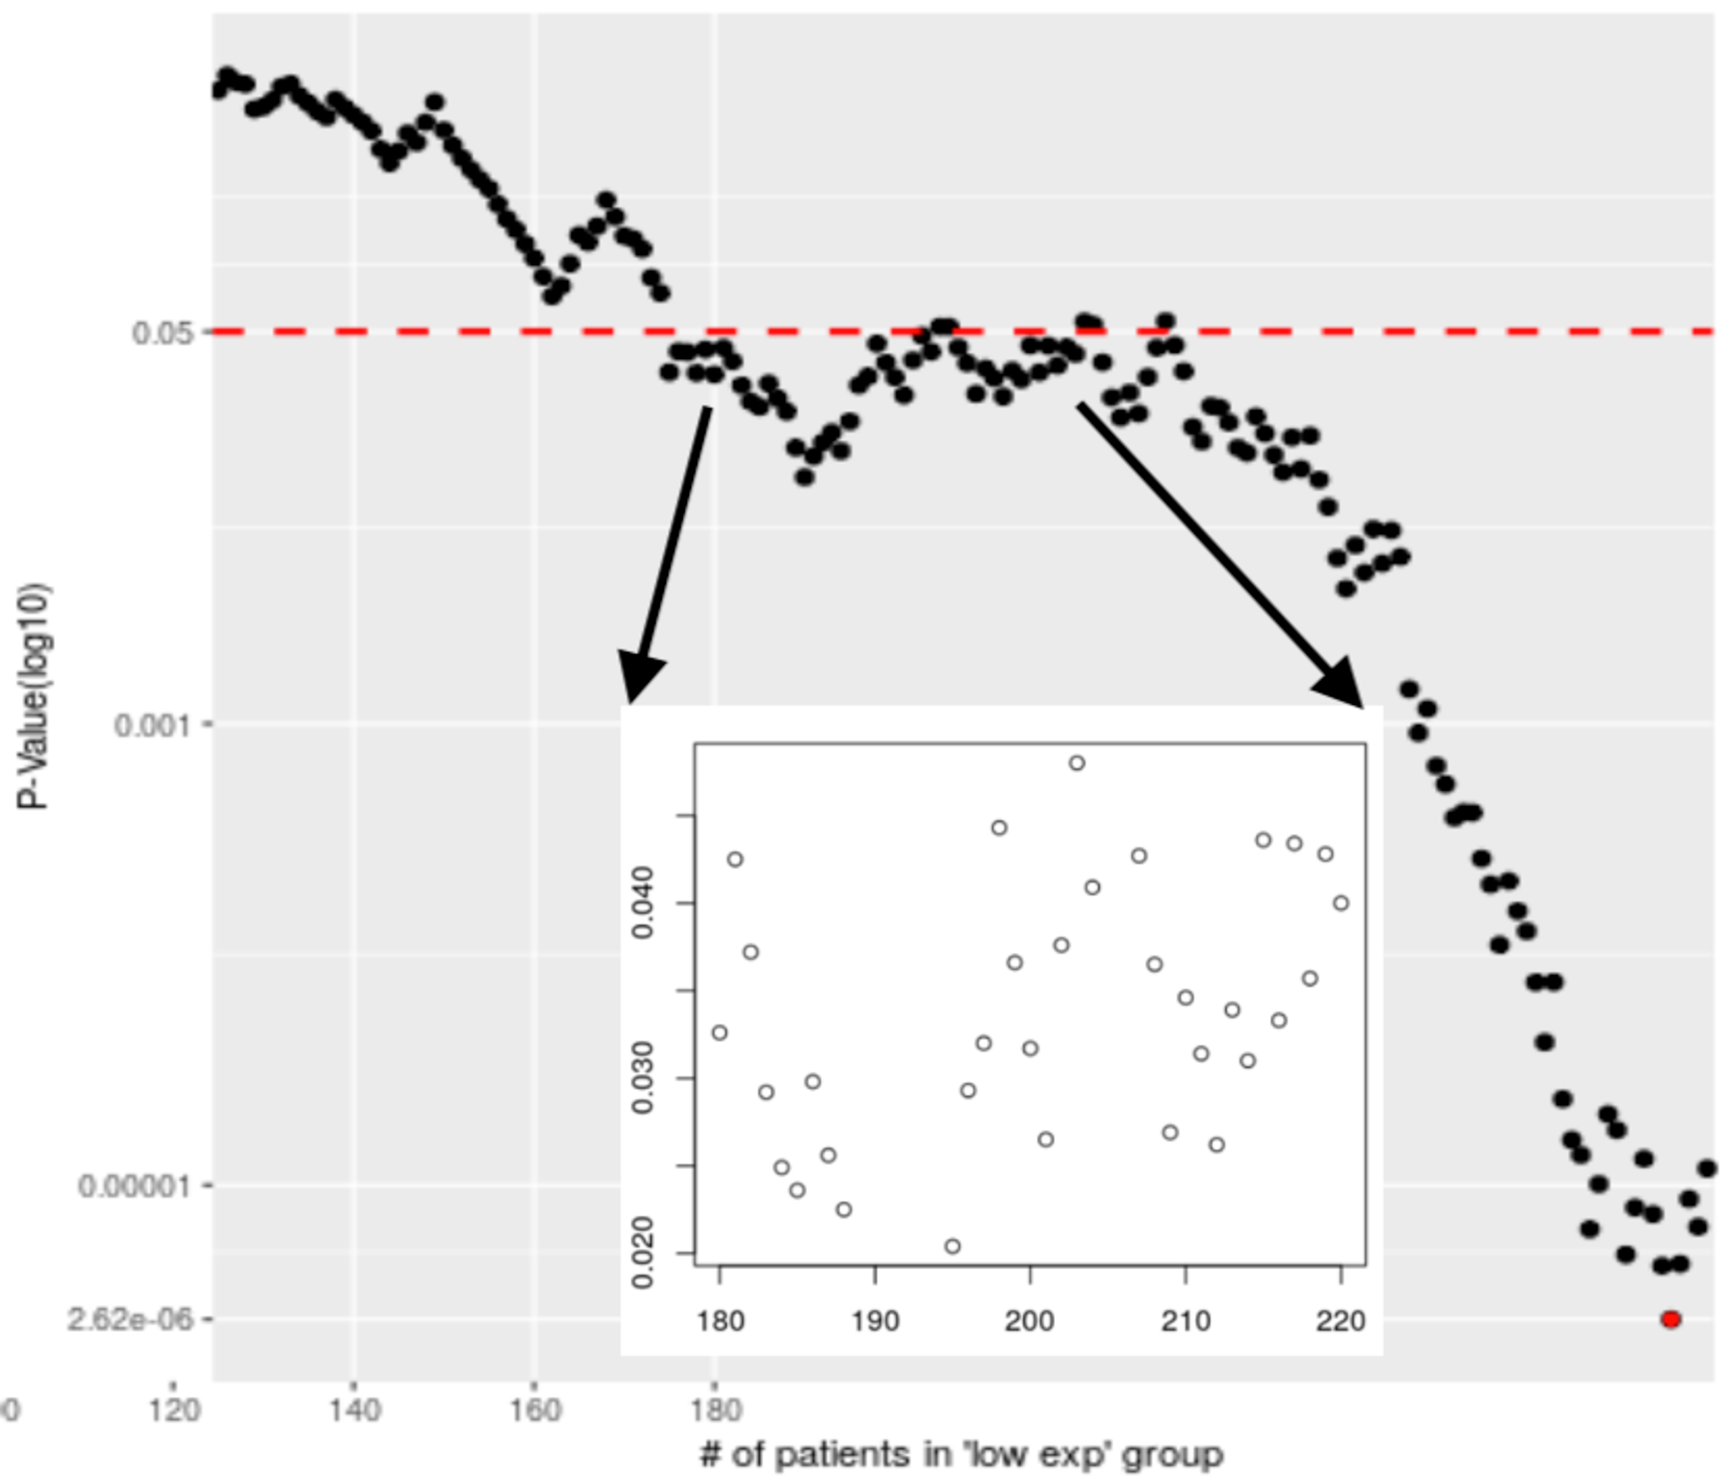
\includegraphics[width=10cm]{Rplot_pvaluePlot_NDFIP1.pdf}
    \caption{Under cutoff-finding procedure of Kaplan-Meier analysis, the \textit{P}-value plot of gene "NDFIP1" shows: 1) 70\% of \textit{P} values is $<0.05$; 2) the median-cut zone (zoom-in and revealed in inset box) has a "W"-like distribution; 3) sliding-window cutoff selection could find it's optimized \textit{P} values (far less than 0.001) while a median cut might yield \textit{P} value $>=0.05$.\\
    (x-axis: grouping by person number; y-axis: \textit{P} value in log10 transformed)}
    \label{fig:pvaluePlot_NDFIP1}
\end{figure}


% S2
% from Answer2-2 GSE2837; 
\begin{figure}
\raggedleft
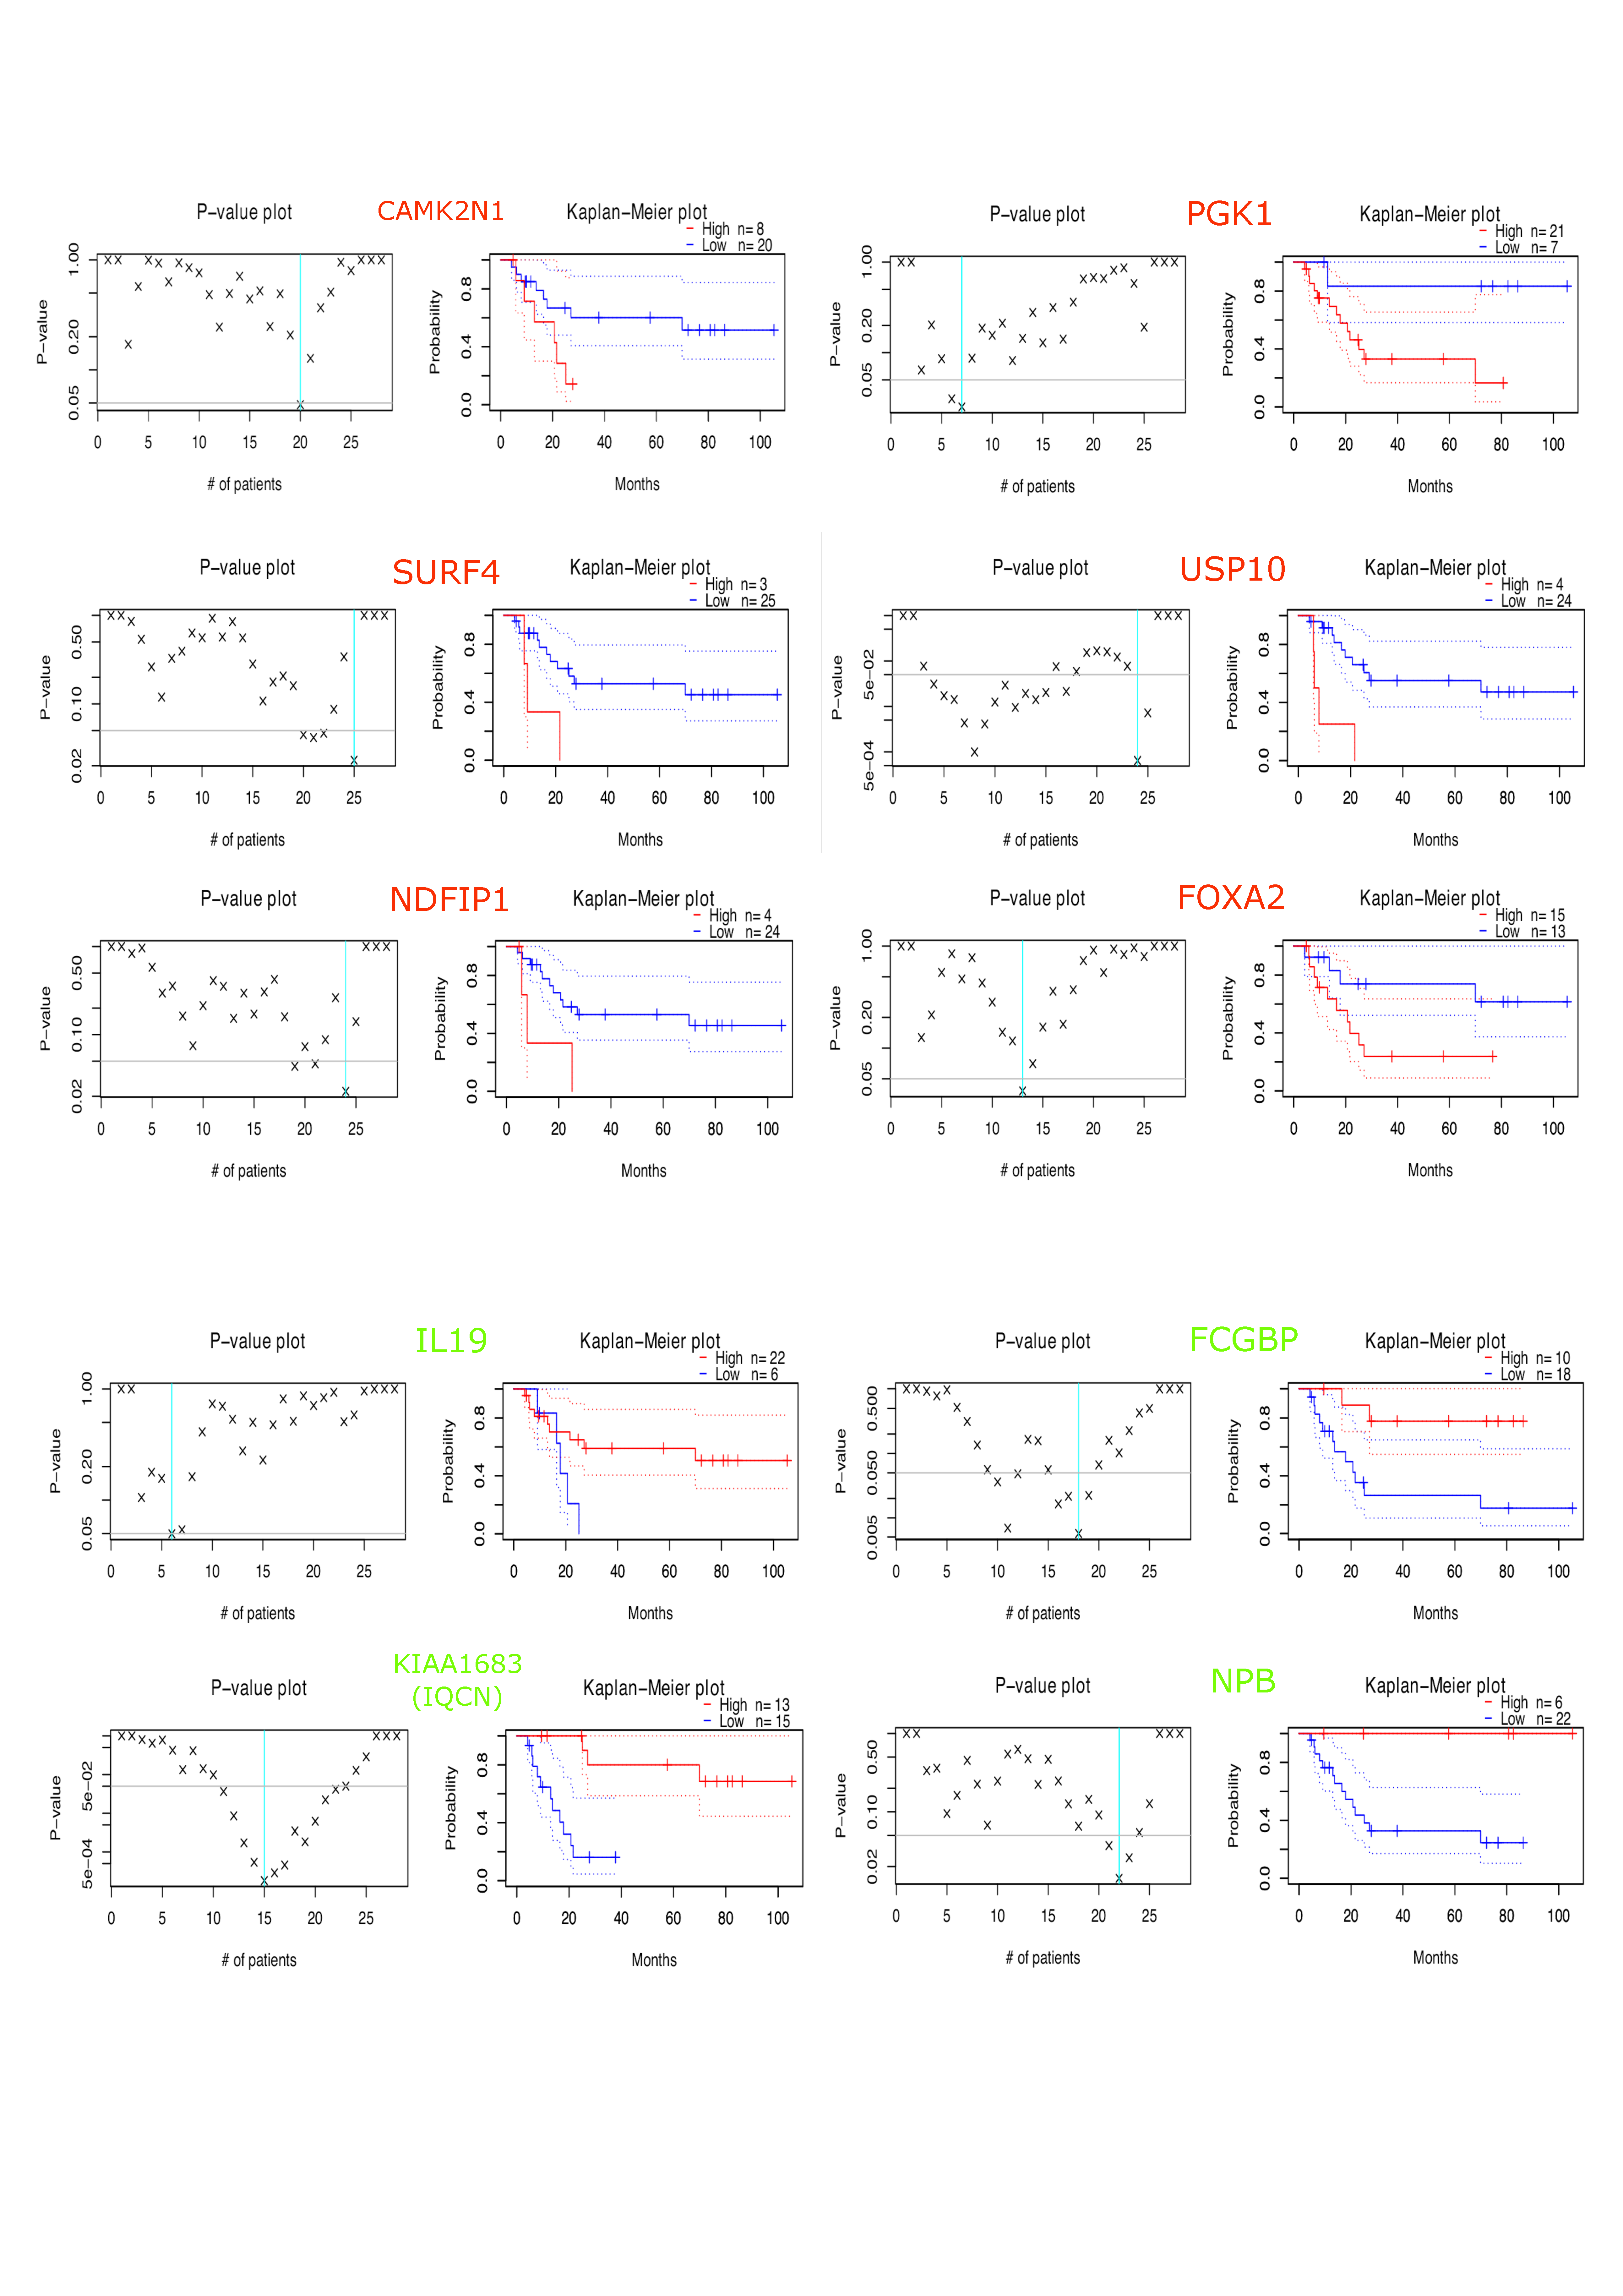
\includegraphics[width=12cm]{Answer_2-2.pdf}
\caption{GSE2837 query results from PrognoScan: Kaplan-Meier plots of 10 genes (the cutoff of \textcolor{red}{high risk} and \textcolor{blue}{low risk} groups, which is derived from cumulative P-value plots). The poor prognostic genes are marked as \textcolor{red}{red}; the better prognostic genes are marked as \textcolor{green}{green}.}
\label{fig:fig_GSE2837}
\end{figure}




%\clearpage

%\bibliographystyle{unsrt} %model1-num-names}
%\bibliography{TCGA_margin_cutoff.bib}

\end{document}

%%%
% MDPI internal command: Title for citation in the left column
\TitleCitation{A Global Genome-wide Scan with Optimal Cutoff Mining for Emerging Biomarkers in Head and Neck Squamous Cell Carcinoma}

% Author Orchid ID: enter ID or remove command
\newcommand{\orcidauthorA}{0000-0002-4476-2600} % Add \orcidA{} behind the author's name
\newcommand{\orcidauthorB}{0000-0001-6497-4232} % Add \orcidB{} behind the author's name

% Authors, for the paper (add full first names)
\Author{
Li-Hsing Chi $^{1,2}$\orcidA{}
, Alexander TH Wu $^{1}$,
Michael Hsiao $^{3}$*
and Yu-Chuan (Jack) Li $^{1,4}$*\orcidB{}
}
%\Author{Firstname Lastname $^{1,\dagger,\ddagger}$\orcidA{}, Firstname Lastname $^{1,\ddagger}$ and Firstname Lastname $^{2,}$*}

% MDPI internal command: Authors, for metadata in PDF
\AuthorNames{Li-Hsing Chi, Alexander TH Wu, Michael Hsiao and Yu-Chuan (Jack) Li}

% MDPI internal command: Authors, for citation in the left column
\AuthorCitation{Chi, LH.; Wu, ATH.; Hsiao, M.; Li, YCJ.}

% Affiliations / Addresses (Add [1] after \address if there is only one affiliation.)
\address{%

$^{1}$ \quad The Ph.D. Program for Translational Medicine, College of Medical Science and Technology\unskip, 
    Taipei Medical University and Academia Sinica\unskip, Taipei\unskip, Taiwan\\
$^{2}$ \quad Division of Oral and Maxillofacial Surgery, Department of Dentistry\unskip,
    Taipei Medical University Hospital\unskip, Taipei\unskip, Taiwan\\
$^{3}$ \quad Genomics Research Center\unskip, 
    Academia Sinica\unskip, Taipei\unskip, Taiwan\\
$^{4}$ \quad Graduate Institute of Biomedical Informatics, College of Medical Science and Technology\unskip, Taipei Medical University\unskip, Taipei\unskip, Taiwan\\
}

% Contact information of the corresponding author
\corres{
Correspondence: Hsiao: mhsiao@gate.sinica.edu.tw; Li: jaak88@gmail.com\\[1cm]
}
%(optional; include country code; if there are multiple corresponding authors, add author initials) +xx-xxxx-xxx-xxxx (F.L.)}


%%

% x SFigure 2, SurvExpress
% red or green is NOT by expression level
\begin{figure}
\raggedleft
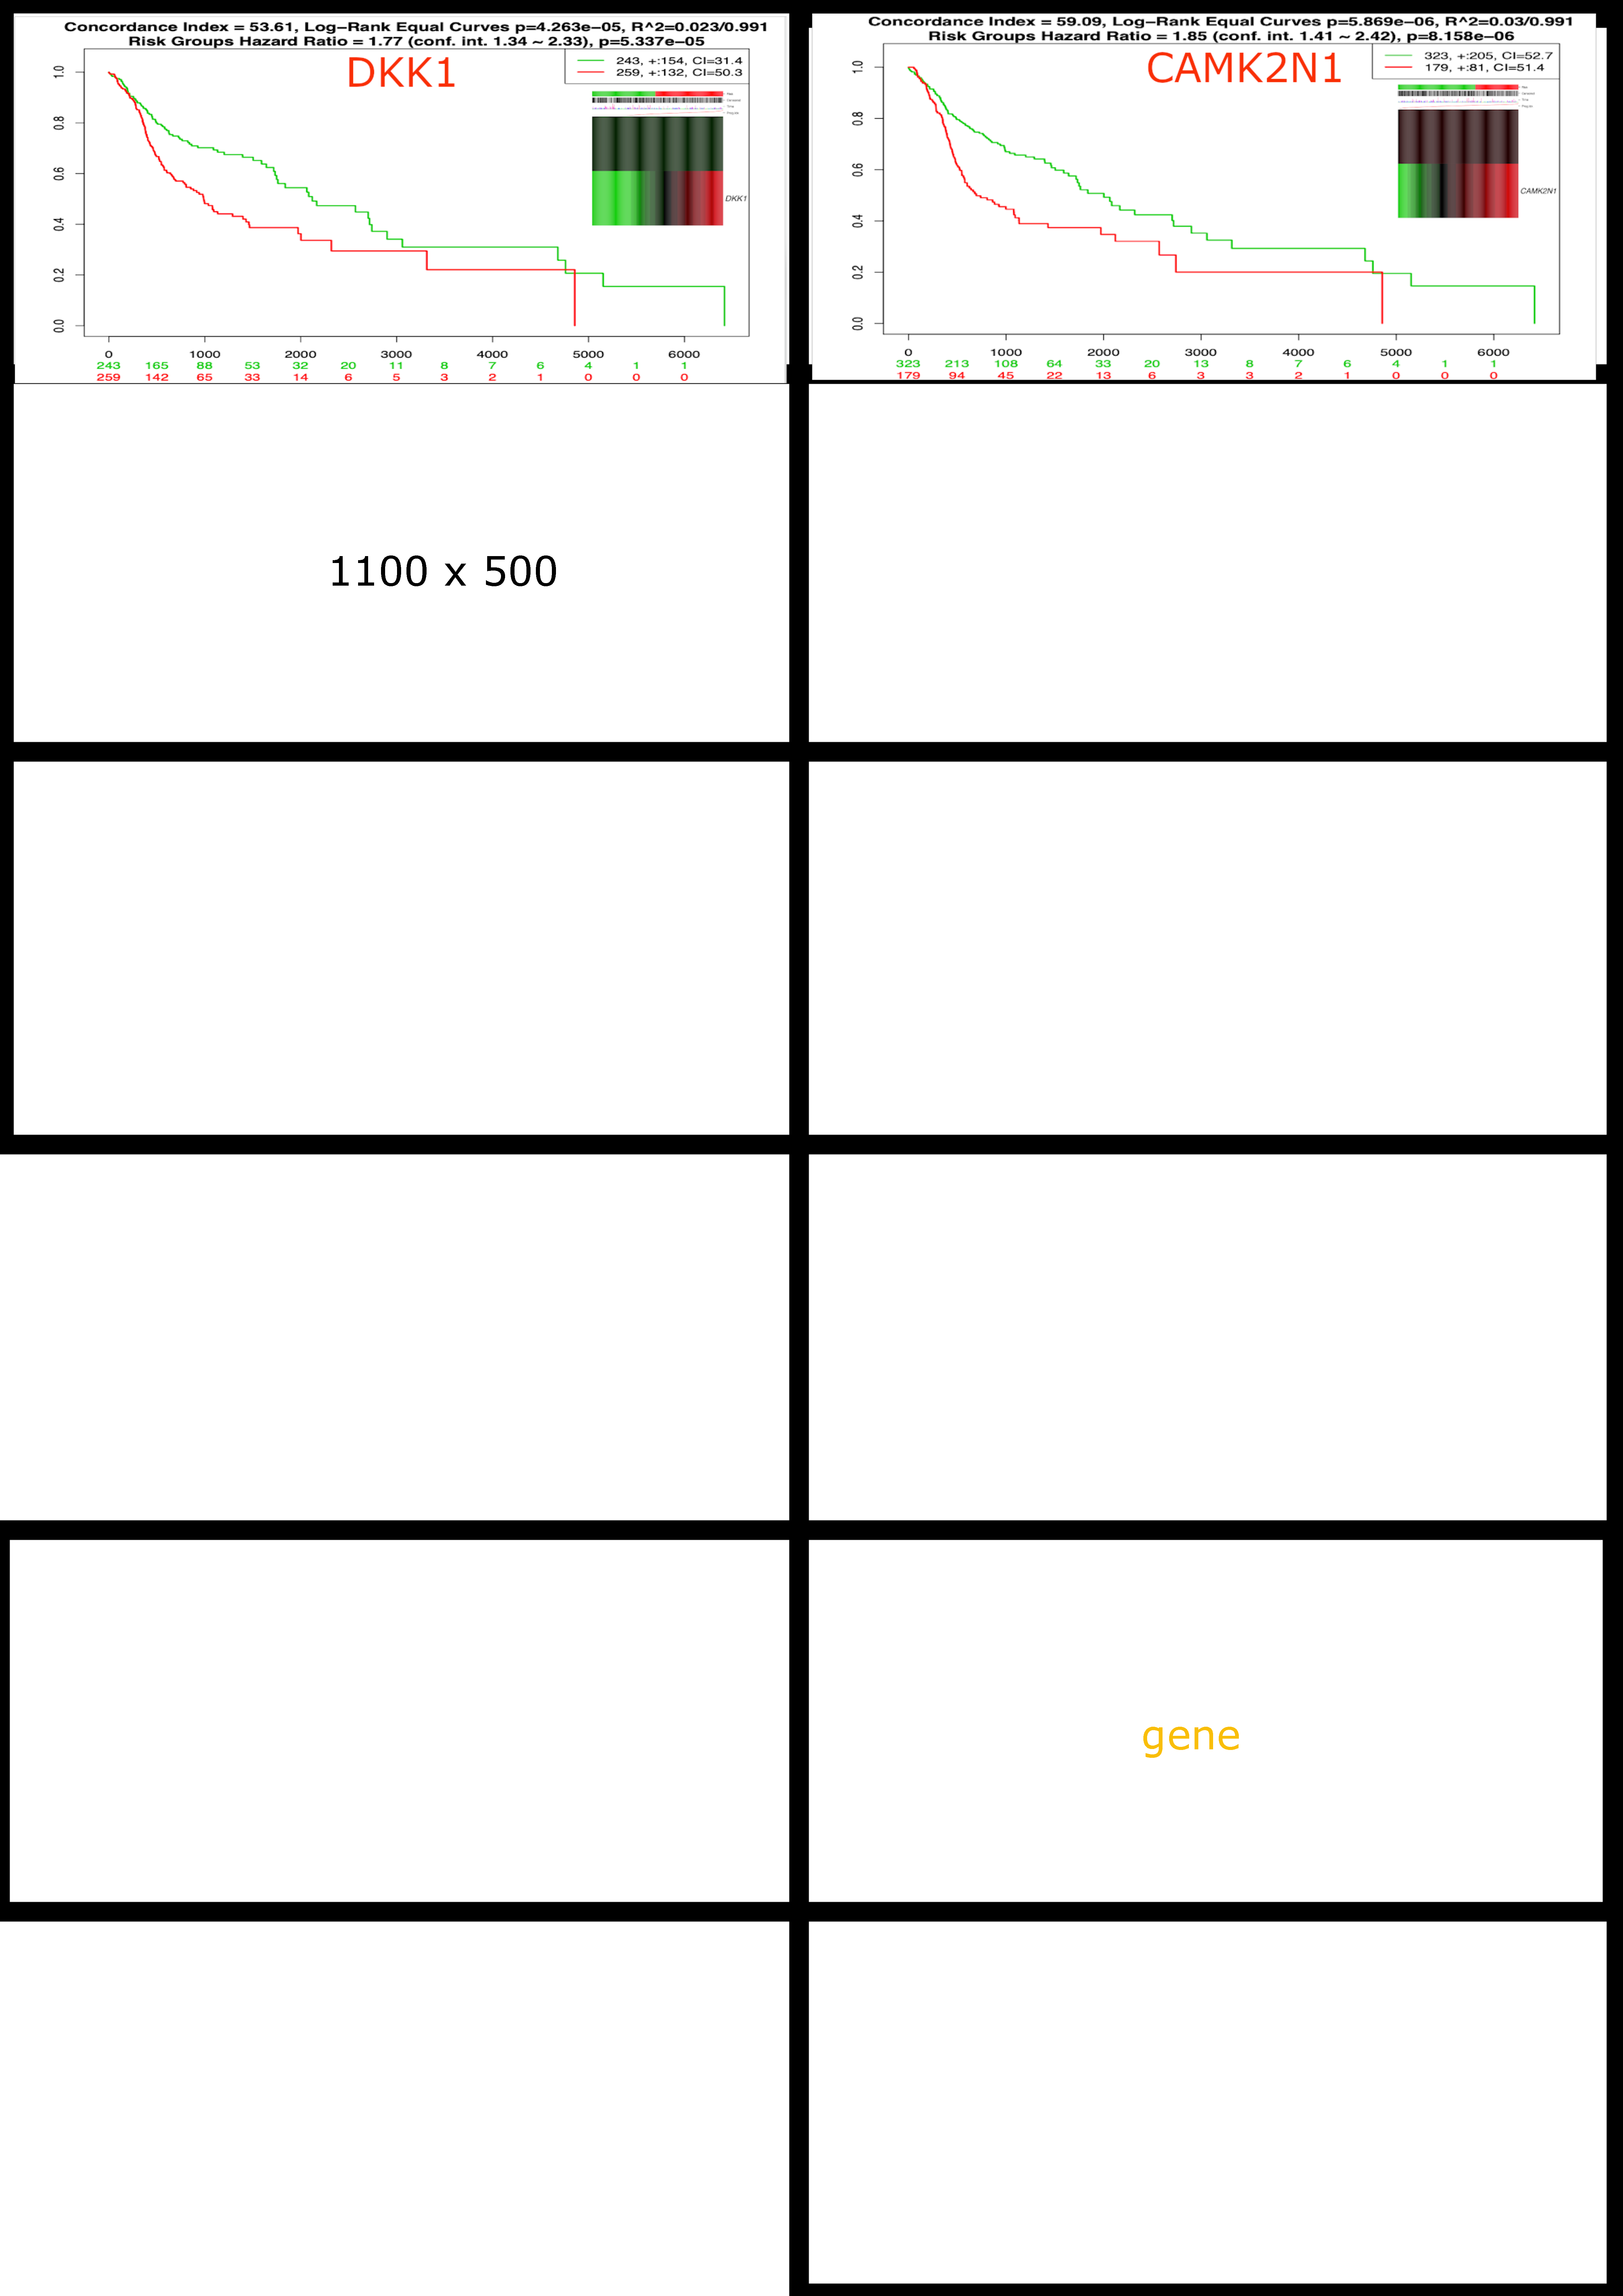
\includegraphics[width=10cm]{Answer_3-1.pdf}
\caption{The query results from SurvExpress: Kaplan-Meier plots of 12 genes (the cutoff of \textcolor{red}{high risk} and \textcolor{green}{low risk} groups, which is derived from risk groups optimization. %cumulative P-value plots).
Inset color scale shows risk groups (\textcolor{red}{high}/\textcolor{green}{low}) and corresponded RNA expression in \textcolor{red}{high}/\textcolor{green}{low}.
Thus, the poor prognostic genes are marked as \textcolor{red}{red}; the better prognostic genes are marked as \textcolor{orange}{orange}.}
\label{fig:fig_SurvExpress}
\end{figure}
\clearpage

%%
%x S3
\begin{figure}
\raggedleft
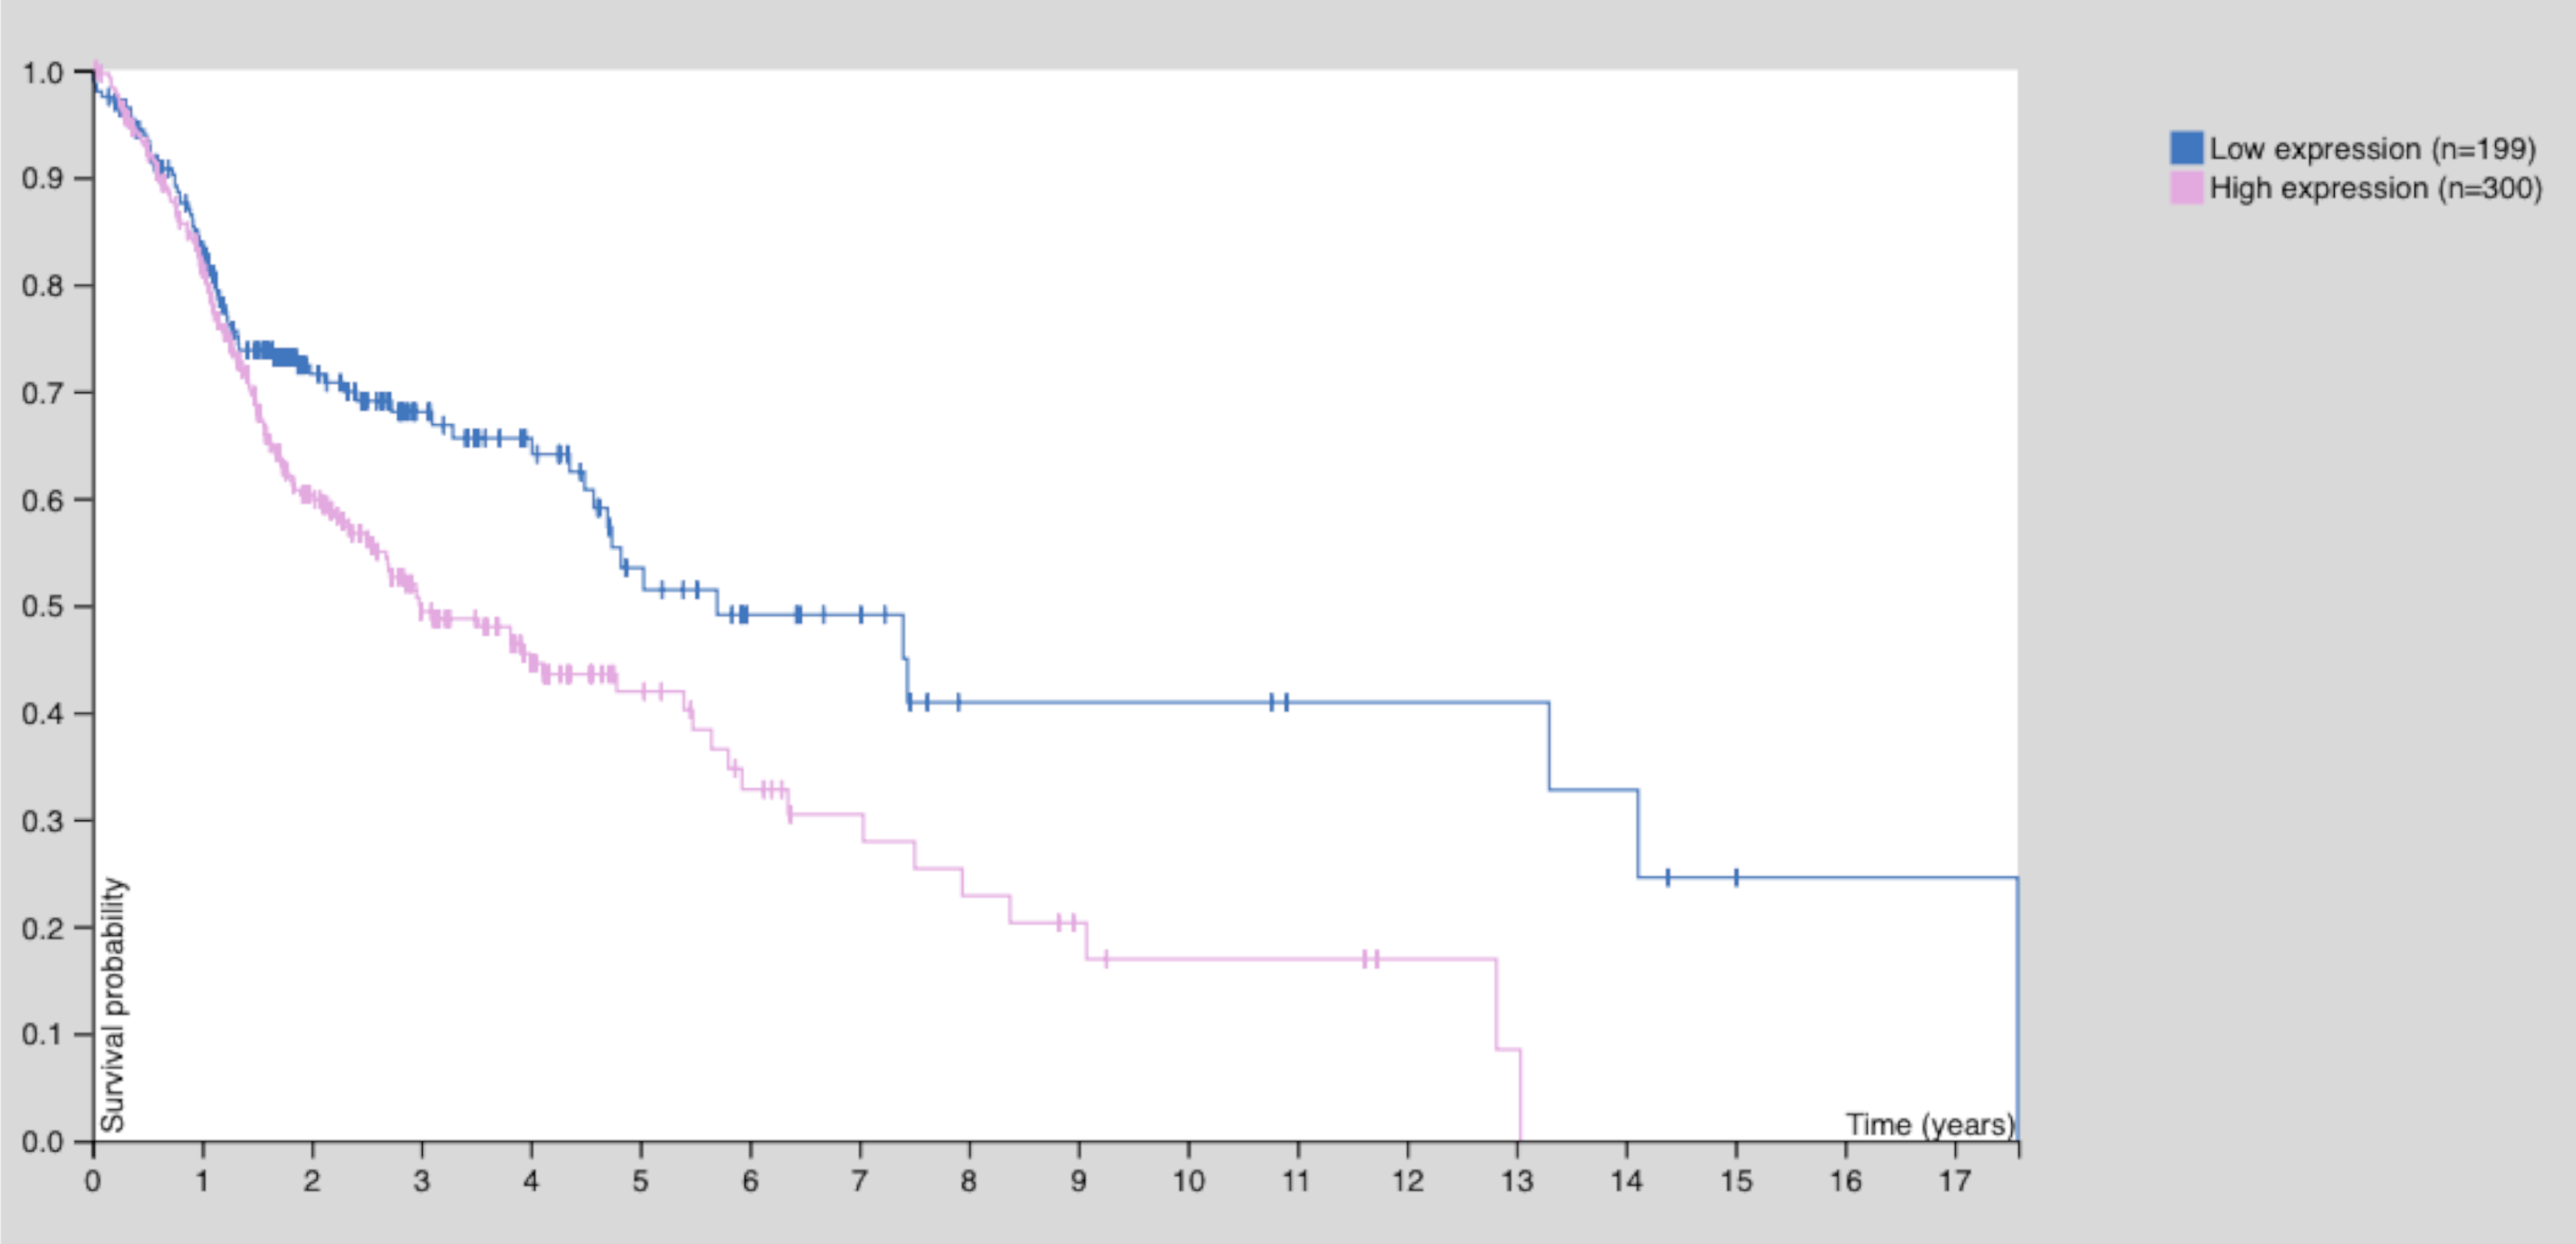
\includegraphics[width=12cm]{Answer_3-1_USP10.pdf}
\caption{The query results from HPA: Kaplan-Meier plots of  ubiquitin specific peptidase 10 (USP10) with cutoff by mRNA \textcolor{red}{high expression} and \textcolor{blue}{low expression} groups (P-value = 0.0018).
Overexpression of USP10 has poor prognosis on HNSCC.}
\label{fig:fig_HPA_USP10}
\end{figure}
%\clearpage
